% !TEX program = xelatex
% !TEX encoding = UTF-8
\documentclass{article}

\usepackage{ifthen}
\newif\ifsolutions
\solutionsfalse

\usepackage[UTF8,fontset=none]{ctex}
\usepackage{graphicx}
\usepackage{booktabs}
\setCJKmainfont{Songti SC}
\setCJKsansfont{Hiragino Sans GB}
\setCJKmonofont{Hiragino Sans GB}

\long\def\dqnAnswerBasic{%
\subsubsection*{环境、算法与评估设置}
CartPole-v1 的状态由小车位置与速度、杆的角度与角速度组成，动作是向左或向右施力。杆保持竖立且小车处于边界内时，每一步获得 $1$ 分；每回合最多 $500$ 步。

所有运行采用两层、每层 $64$ 个单元的 Q 网络，折扣因子 $\gamma=0.99$，batch size 为 $128$，前 $20{,}000$ 步收集经验，每 $1{,}000$ 步同步目标网络。总训练长度为 $300{,}000$ 环境步；每 $10{,}000$ 步评估一次，每次取 $10$ 回合的平均回报。最后一次评估在 $290{,}000$ 步。CartPole 基线与学习率对照采用种子 $1$；LunarLander 采用种子 $1$、$2$、$3$。训练环境按种子初始化，评估环境采用相应种子加 $10{,}000$。

\noindent\begin{minipage}{\linewidth}
\setlength{\intextsep}{4pt}
\setlength{\abovecaptionskip}{4pt}
\subsubsection*{CartPole 基线表现}
\begin{figure}[H]
  \centering
  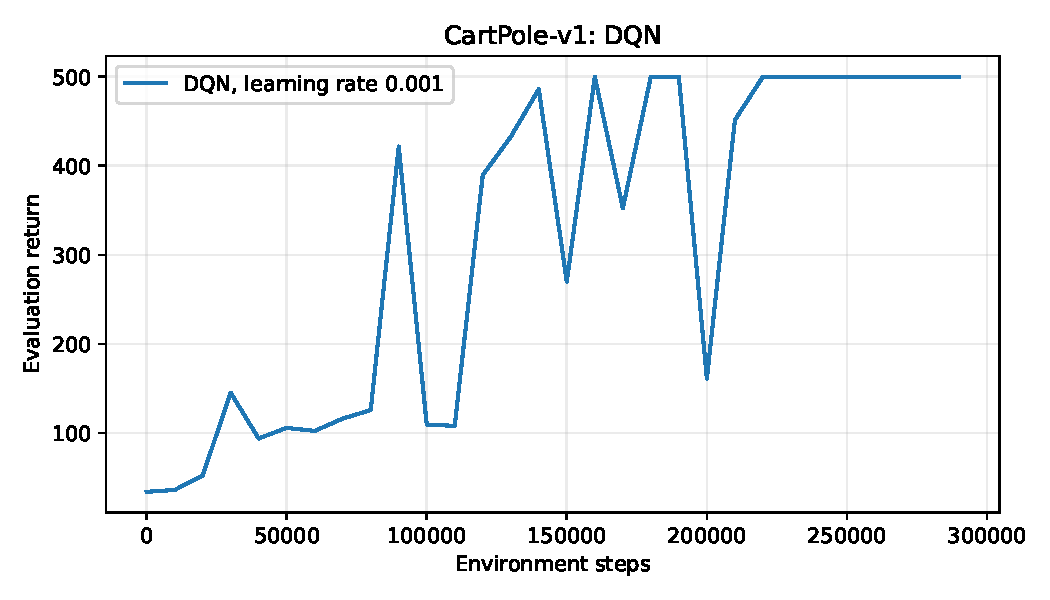
\includegraphics[width=0.74\linewidth]{results/q1/cartpole_eval.pdf}
  \caption{CartPole-v1 基线 DQN 的平均评估回报。横轴为环境步数，纵轴为十回合平均回报；学习率为 $0.001$。}
  \label{fig:cartpole}
\end{figure}

如图~\ref{fig:cartpole} 所示，基线在 $220{,}000$ 步之后的各次评估均为 $500$ 分。中段曲线仍有波动，后段则连续保持满分，说明该次训练最终形成了能维持整回合平衡的策略。

\end{minipage}\par\medskip
\noindent\begin{minipage}{\linewidth}
\setlength{\intextsep}{4pt}
\setlength{\abovecaptionskip}{4pt}
\subsubsection*{LunarLander 三个种子的结果}
\begin{figure}[H]
  \centering
  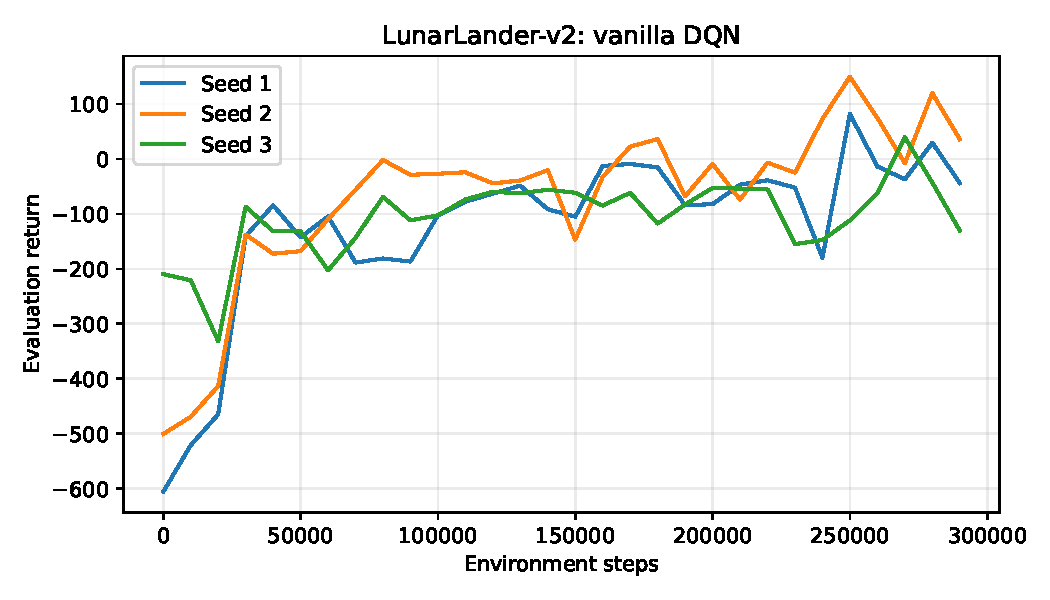
\includegraphics[width=0.74\linewidth]{results/q1/lunarlander_three_seeds.pdf}
  \caption{LunarLander-v2 上普通 DQN 的三个独立种子。每个点是十回合的平均评估回报。}
  \label{fig:lunar}
\end{figure}

\begin{table}[H]
  \centering
  \caption{LunarLander-v2 的评估回报}
  \begin{tabular}{ccc}
    \toprule
    种子 & 最后一次评估 & 训练期间最高评估 \\
    \midrule
    1 & $-43.8$ & $81.9$ \\
    2 & $35.7$ & $149.5$ \\
    3 & $-130.4$ & $39.3$ \\
    \bottomrule
  \end{tabular}
  \label{tab:lunar}
\end{table}

\end{minipage}\par\medskip
\noindent\begin{minipage}{\linewidth}
\subsubsection*{学习率 $0.05$ 对 Q 估计的影响}
\begin{figure}[H]
  \centering
  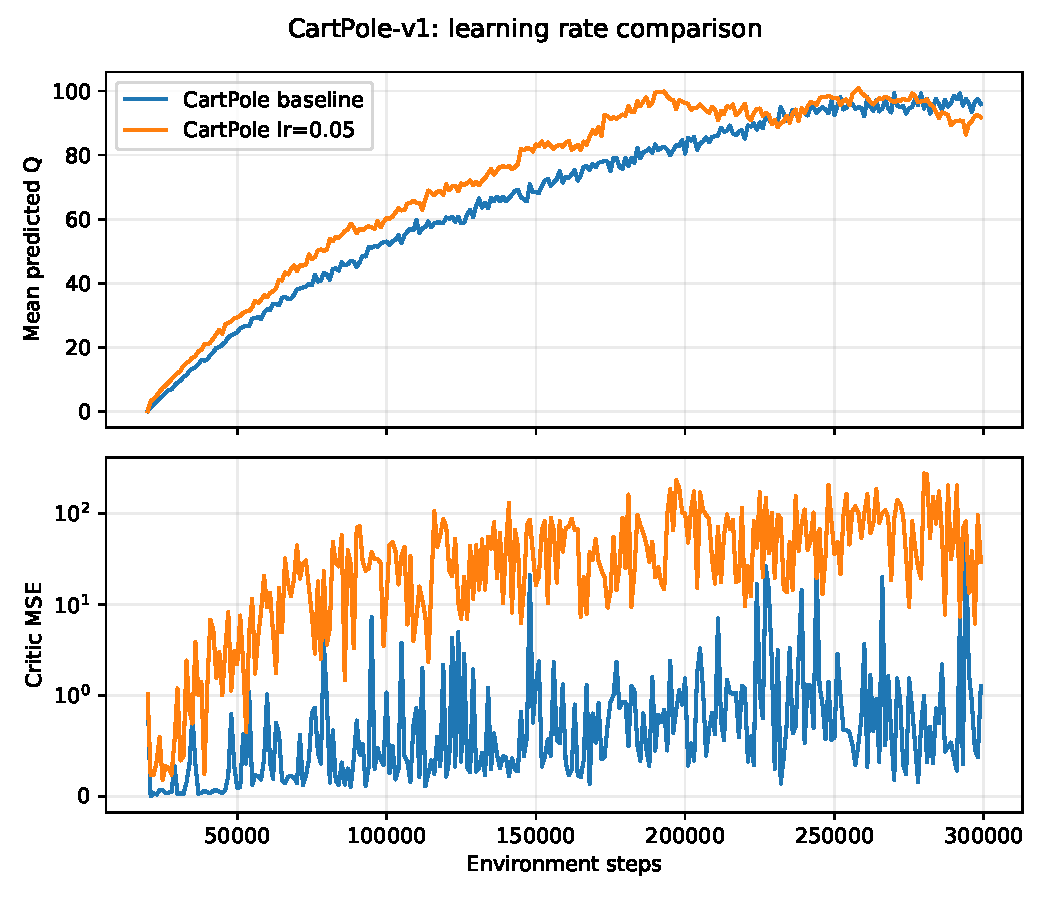
\includegraphics[width=0.85\linewidth]{results/q1/cartpole_learning_rate.pdf}
  \caption{CartPole-v1 在学习率 $0.001$ 与 $0.05$ 下的预测 Q 值和 critic 均方误差。预测 Q 值为回放 batch 中所选动作的均值；下图采用对称对数纵轴，以展示误差的跨度。}
  \label{fig:lr-critic}
\end{figure}

图~\ref{fig:lr-critic} 中，学习率 $0.05$ 的预测 Q 值上升至约 $90$--$100$；critic 误差增大且波动加剧，其中位数由基线的 $0.51$ 升至 $30.74$。最后评估回报由基线的 $500$ 降至 $75$。

DQN 使用当前网络拟合由目标网络构造的自举目标。较大的学习率增大参数更新幅度，使 Q 估计更容易偏离目标；估值误差又通过自举进入后续更新，从而放大训练波动。这对应课堂中函数近似、离策略学习与自举共同作用的“致命三要素”：本实验中的表现是 critic 误差增大、估值波动和策略回报下降。
\end{minipage}\par\medskip
}

\long\def\dqnAnswerDoubleQ{%
\noindent\begin{minipage}{\linewidth}
\subsubsection*{Double Q 与普通 DQN 的 LunarLander 对照}
Double Q 使用在线网络选择下一动作 $a'=\arg\max_a Q_{\phi}(s',a)$，再由目标网络计算 $Q_{\phi'}(s',a')$，并构造目标 $y=r+\gamma(1-d)Q_{\phi'}(s',a')$。分离动作选择与估值，能够减弱最大值运算对估值噪声的放大。

\begin{figure}[H]
  \centering
  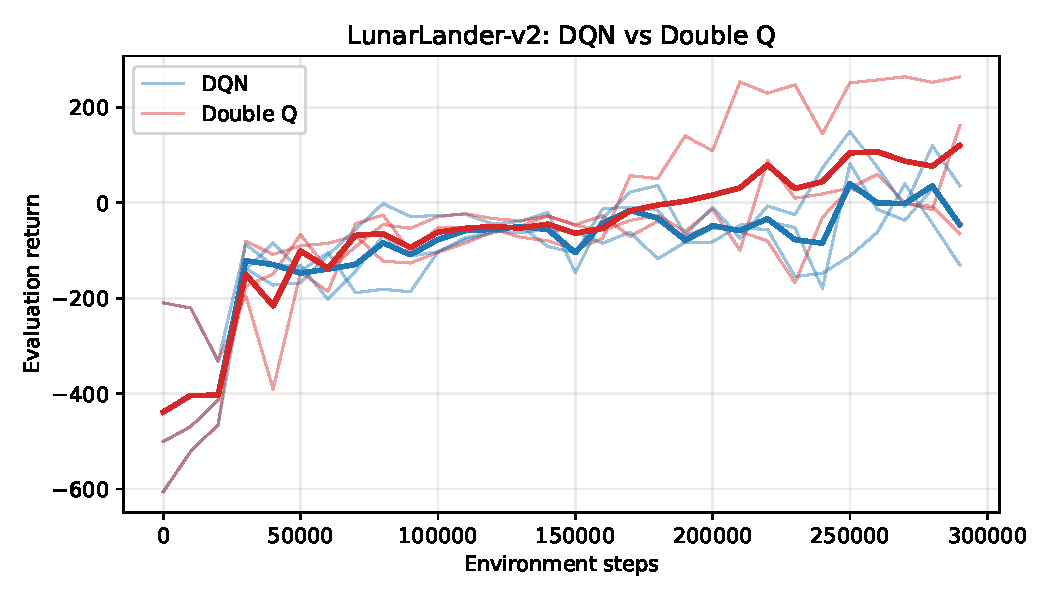
\includegraphics[width=0.88\linewidth]{results/q1/lunarlander_doubleq_comparison.pdf}
  \caption{LunarLander-v2 中普通 DQN（蓝）与 Double Q（红）的三个种子评估回报。细线表示各个种子，粗线表示三个种子的平均值；横轴为环境步数。}
  \label{fig:doubleq-lunar}
\end{figure}

\begin{table}[H]
  \centering
  \caption{LunarLander-v2 各种子的最后一次评估回报}
  \begin{tabular}{ccc}
    \toprule
    种子 & 普通 DQN & Double Q \\
    \midrule
    1 & $-43.8$ & $161.9$ \\
    2 & $35.7$ & $-65.0$ \\
    3 & $-130.4$ & $263.6$ \\
    三种子均值 & $-46.2$ & $120.2$ \\
    \bottomrule
  \end{tabular}
  \label{tab:doubleq-lunar}
\end{table}

Double Q 在种子 1 和 3 上提高了末次回报，在种子 2 上降低了回报；三个种子的末次均值由 $-46.2$ 升至 $120.2$。图~\ref{fig:doubleq-lunar} 中，后期红线的均值整体高于蓝线。普通 DQN 对同一组带噪声的目标估值执行最大化，容易选中被高估的动作；Double Q 分离动作选择与估值，减弱这种过估计反馈，从而改善后期回报。

\end{minipage}\par\medskip
\noindent\begin{minipage}{\linewidth}
\subsubsection*{MsPacman 的训练回报与评估回报}
按 \texttt{mspacman.yaml} 在 \texttt{MsPacmanNoFrameskip-v0} 上训练 $1{,}000{,}000$ 环境步，启用 Double Q、四帧堆叠、四步跳帧与灰度输入。batch size 为 $8$，每 $4$ 环境步更新一次；学习率为 $10^{-4}$，目标网络每 $2{,}000$ 步同步。

\begin{figure}[H]
  \centering
  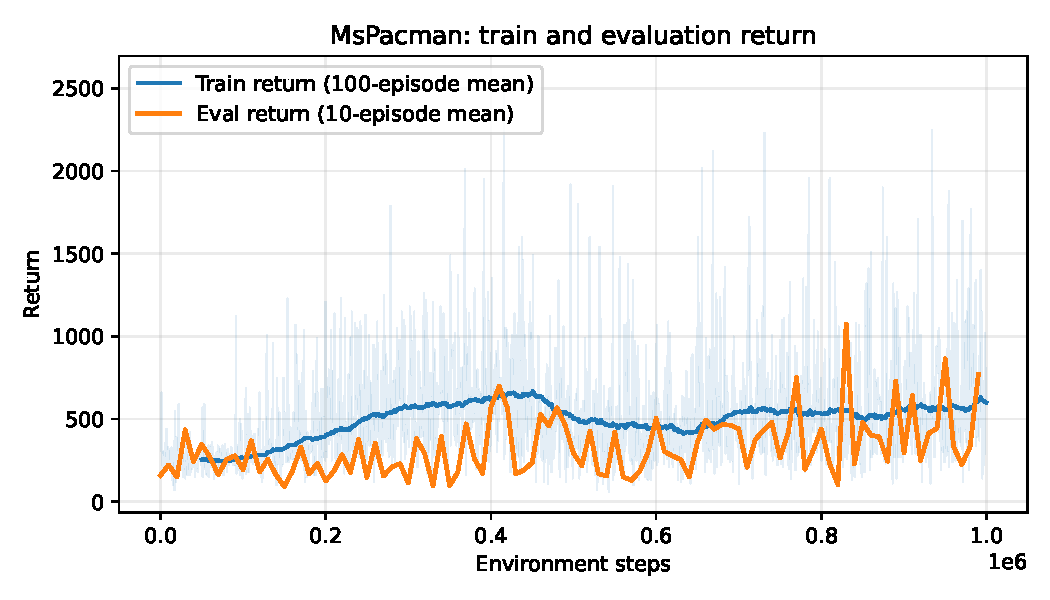
\includegraphics[width=0.88\linewidth]{results/q1/mspacman_train_eval.pdf}
  \caption{MsPacman 的训练回报与评估回报。浅蓝线为每回合训练回报，深蓝线为最近 $100$ 个训练回合的滑动均值，橙线为每次 $10$ 回合的平均评估回报。横轴为环境步数。}
  \label{fig:mspacman-return}
\end{figure}

训练回报的最近 $100$ 回合均值由最初约 $255$ 增至最后约 $600$；评估回报波动较大，在 $830{,}000$ 步达到 $1{,}074$，末次为 $769$。前期两条曲线的差别来自采样策略：训练时 $\epsilon$ 在前 $20{,}000$ 步保持 $1$，随后逐渐下降，评估时固定为 $0.02$。因此，训练轨迹包含较多探索动作，而评估曲线主要反映当时接近贪心的策略。图中训练均值跨 $100$ 回合，评估均值每点仅跨 $10$ 回合，后者也因此更容易出现短期波动。

\end{minipage}\par\medskip
}

\long\def\dqnAnswerHyperparams{%
\noindent\begin{minipage}{\linewidth}
\subsubsection*{四档学习率的敏感性}
\begin{figure}[H]
  \centering
  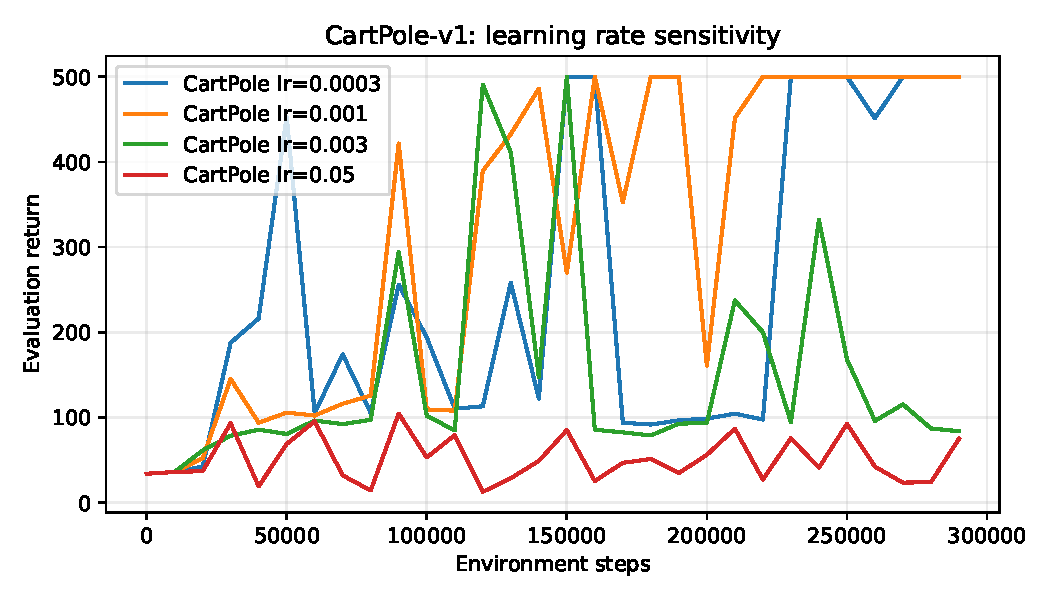
\includegraphics[width=0.88\linewidth]{results/q1/cartpole_four_learning_rates.pdf}
  \caption{CartPole-v1 的四档学习率对照。选择学习率，是因为它直接控制每次 Q 网络更新的幅度，可以检验自举目标下训练表现对更新步长的敏感性。四条曲线均使用种子 $1$。}
  \label{fig:four-lr}
\end{figure}

\begin{table}[H]
  \centering
  \caption{四档学习率的评估回报}
  \begin{tabular}{ccc}
    \toprule
    学习率 & 最后一次评估 & 训练期间最高评估 \\
    \midrule
    $0.0003$ & $500.0$ & $500.0$ \\
    $0.001$ & $500.0$ & $500.0$ \\
    $0.003$ & $83.8$ & $500.0$ \\
    $0.05$ & $75.0$ & $104.6$ \\
    \bottomrule
  \end{tabular}
  \label{tab:four-lr}
\end{table}

图~\ref{fig:four-lr} 与表~\ref{tab:four-lr} 中，学习率 $0.0003$ 与 $0.001$ 的末次回报均为 $500$；$0.003$ 达到过 $500$ 后回落至 $83.8$；$0.05$ 的最高回报为 $104.6$。在这四档设置中，$0.0003$ 与 $0.001$ 的训练结束表现最好。
\end{minipage}\par\medskip
}

\long\def\sacAnswerReinforce{%
\paragraph{实验设置与回报曲线}
在 HalfCheetah-v4 上分别使用单样本和十样本 REINFORCE，均训练 $1{,}000{,}000$ 个环境步。两组实验采用种子 $1$、$128$ 个样本的回放 batch、折扣因子 $0.99$、熵系数 $0.2$，每 $10{,}000$ 步评估十个回合。图~\ref{fig:sac-reinforce} 的纵轴为十回合平均评估回报。
\begin{figure}[H]
  \centering
  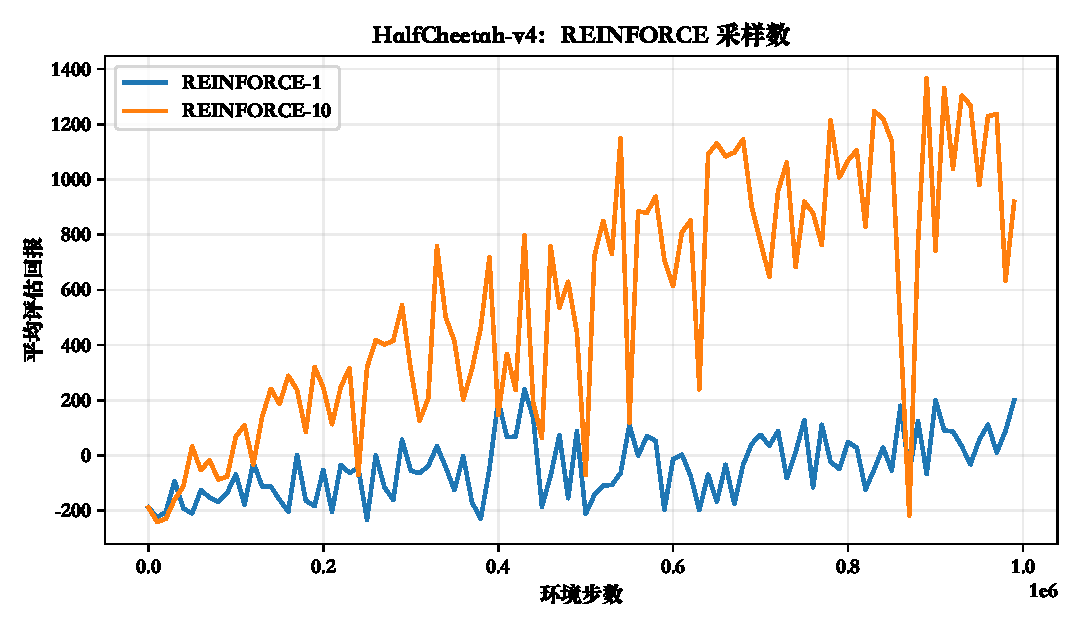
\includegraphics[width=0.9\linewidth]{results/q2/halfcheetah_reinforce.pdf}
  \caption{HalfCheetah-v4 上 REINFORCE-1 与 REINFORCE-10 的评估回报。}
  \label{fig:sac-reinforce}
\end{figure}
图~\ref{fig:sac-reinforce} 中，REINFORCE-10 的后期回报整体高于 REINFORCE-1；在最后一次 $990{,}000$ 步评估中，两者分别为 $919.4$ 和 $200.4$。两组使用相同的网络、优化器与熵系数，差别在于每个回放状态采样的动作数。REINFORCE-10 对十个动作的 $\nabla_\theta\log\pi_\theta(a\mid s)Q(s,a)$ 取平均，降低动作采样引入的梯度方差，使策略更新方向更稳定，因此取得了更高的回报。
}

\long\def\sacAnswerReparametrize{%
\paragraph{三种 actor 梯度估计的比较}
重参数化实验训练 $1{,}000{,}000$ 环境步，种子、回放 batch 和评估频率与两组 REINFORCE 相同。三组均使用三层、每层 $128$ 单元的网络，actor 与 critic 学习率为 $3\times10^{-4}$，目标网络软更新系数为 $0.005$；重参数化的熵系数为 $0.1$，REINFORCE 为 $0.2$。
\begin{figure}[H]
  \centering
  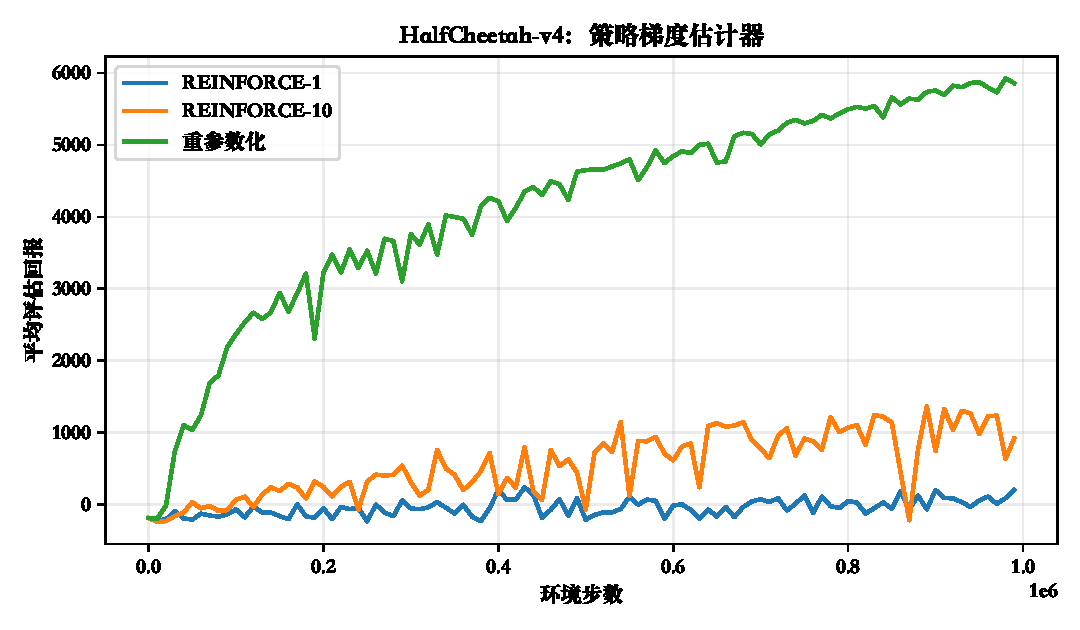
\includegraphics[width=0.9\linewidth]{results/q2/halfcheetah_eval.pdf}
  \caption{HalfCheetah-v4 上三种 actor 梯度估计器的评估回报；横轴为环境步数。}
  \label{fig:sac-halfcheetah}
\end{figure}
\begin{table}[H]
  \centering
  \caption{HalfCheetah-v4 在相同环境步数下的十回合平均评估回报}
  \begin{tabular}{rrrr}
    \toprule
    环境步数 & REINFORCE-1 & REINFORCE-10 & 重参数化 \\
    \midrule
    $100{,}000$ & $-67.9$ & $68.7$ & $2369.6$ \\
    $300{,}000$ & $-54.4$ & $312.7$ & $3760.1$ \\
    $500{,}000$ & $-211.3$ & $-70.3$ & $4649.5$ \\
    $990{,}000$ & $200.4$ & $919.4$ & $5858.8$ \\
    \bottomrule
  \end{tabular}
  \label{tab:sac-halfcheetah}
\end{table}
图~\ref{fig:sac-halfcheetah} 与表~\ref{tab:sac-halfcheetah} 中，重参数化学习最快，在 $100{,}000$ 步达到 $2369.6$，末次回报为 $5858.8$；REINFORCE-10 次之，REINFORCE-1 最低。重参数化通过 \texttt{rsample()} 保留动作对策略参数的可微关系，直接利用 critic 对动作的梯度更新策略；相比 REINFORCE 的分数函数估计，它以更少动作样本获得低方差梯度，提高了环境样本利用效率。

\paragraph{Humanoid-v4}
使用给定的两 critic、最小值目标与重参数化配置，在 $500{,}000$ 个环境步处截断训练。每 $10{,}000$ 步对十个回合计算一次平均评估回报。图~\ref{fig:sac-humanoid} 展示这段训练的评估曲线。
实验采用种子 $1$、三层每层 $256$ 单元的网络、$256$ 个样本的回放 batch、折扣因子 $0.99$、熵系数 $0.05$ 和软更新系数 $0.005$。
\begin{figure}[H]
  \centering
  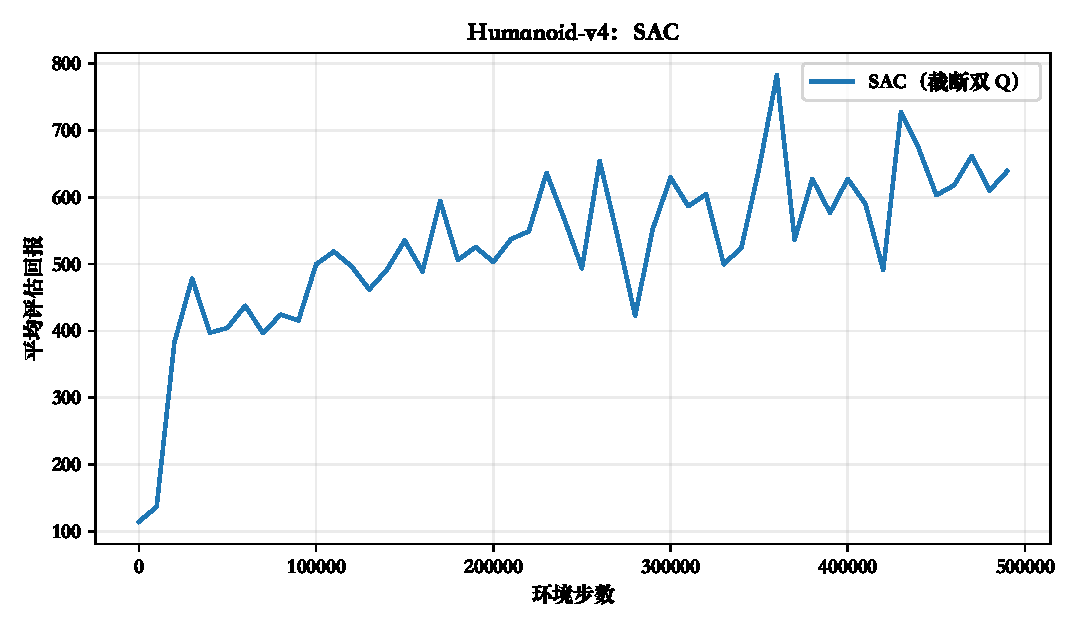
\includegraphics[width=0.9\linewidth]{results/q2/humanoid_eval.pdf}
  \caption{Humanoid-v4 上 clipped double Q SAC 的平均评估回报。}
  \label{fig:sac-humanoid}
\end{figure}
最后一次评估位于 $490{,}000$ 步，十回合平均回报为 $638.9$，训练期间最高评估回报为 $782.2$。
}

\long\def\sacAnswerBonus{%
\paragraph{Hopper-v4 的目标估值对照}
本次运行中，Double Q 的后段平均评估回报最高。三种方法均采用种子 $1$，训练 $100{,}000$ 个环境步；每 $5{,}000$ 步评估十个回合，每 $1{,}000$ 步记录一次回放 batch 的 Q 值均值。网络为三层、每层 $128$ 个单元，batch size 为 $256$，actor 与 critic 学习率均为 $3\times10^{-4}$，$\gamma=0.99$，$\tau=0.005$，熵系数为 $0.05$。按给定 Hopper 配置，actor 使用熵奖励，critic 的自举目标不加入熵项。

Single Q 使用单个目标 critic；Double Q 让两条 critic 交叉使用对方的目标估值；clipped double Q 将两个目标估值的较小值作为共同目标。三种方法的 actor 均使用重参数化更新；双 critic 的 actor 按模板实现使用两条在线 critic 的均值。
\begin{figure}[H]
  \centering
  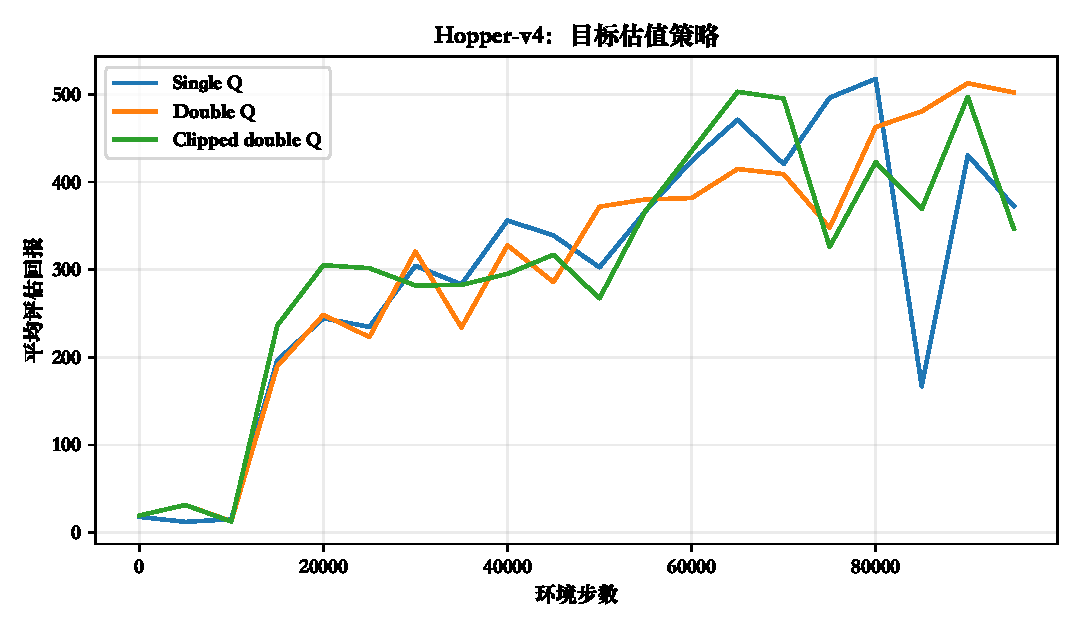
\includegraphics[width=0.9\linewidth]{results/q2/bonus_hopper_return.pdf}
  \caption{Hopper-v4 三种目标策略的十回合平均评估回报。}
  \label{fig:bonus-hopper-return}
\end{figure}
\begin{figure}[H]
  \centering
  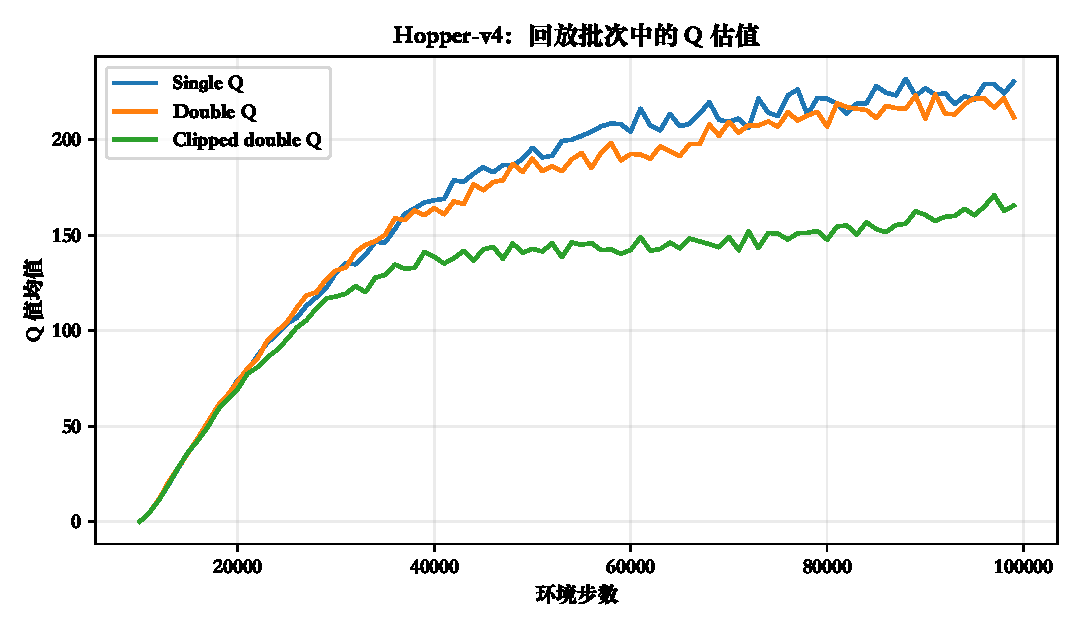
\includegraphics[width=0.9\linewidth]{results/q2/bonus_hopper_q.pdf}
  \caption{Hopper-v4 训练日志中的 \texttt{q\_values}：每次记录为回放 batch 中状态动作对的在线 Q 值均值，双 critic 另对网络取平均。}
  \label{fig:bonus-hopper-q}
\end{figure}
\begin{table}[H]
  \centering
  \caption{Hopper-v4 的回报与估值对照}
  \begin{tabular}{lrrr}
    \toprule
    方法 & 末次评估回报 & 后五次评估均值 & 末次 Q 均值 \\
    \midrule
    Single Q & $372.7$ & $396.9$ & $230.4$ \\
    Double Q & $502.5$ & $461.4$ & $211.7$ \\
    Clipped double Q & $346.9$ & $392.5$ & $165.5$ \\
    \bottomrule
  \end{tabular}
  \label{tab:bonus-hopper}
\end{table}
以后五次评估（$75{,}000$--$95{,}000$ 步）的平均回报比较，Double Q 的 $461.4$ 最高，因此选择 Double Q 进行 Humanoid 实验。表中末次评估发生在 $95{,}000$ 步，末次 Q 记录发生在 $99{,}000$ 步。

图~\ref{fig:bonus-hopper-q} 中，single Q 的末次估值为 $230.4$，高于 Double Q 的 $211.7$，而后段评估回报低于 Double Q。过估计会让 actor 偏向被高估的动作，并通过自举继续放大估值误差；Double Q 交叉使用目标网络，减弱单个 critic 对自身估值误差的反馈。Clipped double Q 取两个目标估值的最小值，使末次 Q 均值降至 $165.5$，体现了最小值目标对估值的抑制作用。其后段回报为 $392.5$，说明更保守的估值在这组实验中对应较低的策略回报，Double Q 的回报表现最好。

\paragraph{Humanoid-v4 的样本效率比较}
采用 Hopper 中回报最好的 Double Q，在 Humanoid-v4 上训练 $500{,}000$ 个环境步。使用三层、每层 $256$ 单元的网络、$256$ 样本的回放 batch、$\gamma=0.99$、$\tau=0.005$ 和熵系数 $0.05$。

同策略对照使用第二次作业的 PGAgent 补跑，采用 reward-to-go、值函数基线、GAE（$\lambda=0.95$）和优势标准化；每批约 $5{,}000$ 个新环境步进行一次 actor 更新和 $50$ 次基线更新。策略和基线均为三层、每层 $256$ 单元，学习率分别为 $3\times10^{-4}$ 和 $10^{-3}$，折扣因子为 $0.99$。两组均采用种子 $1$，以随机策略评估十个回合；横轴为训练环境步数。
\begin{figure}[H]
  \centering
  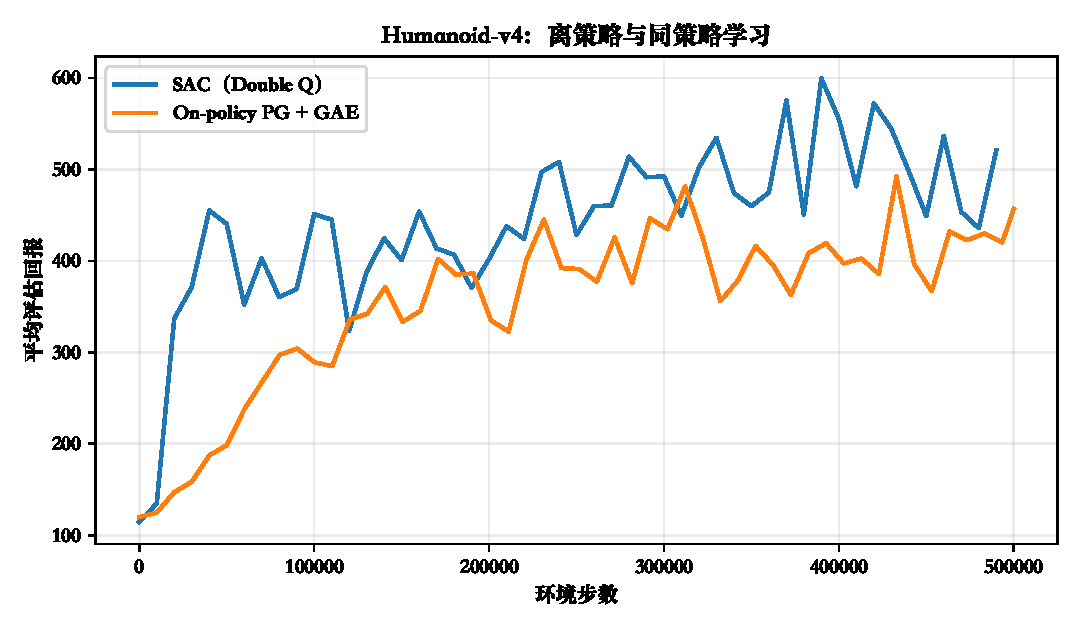
\includegraphics[width=0.9\linewidth]{results/q2/bonus_humanoid_comparison.pdf}
  \caption{Humanoid-v4：按 Hopper 后段回报选择的 Double Q SAC，与本次补跑的同策略 PG+GAE 对照。横轴为各自实际采集的训练环境步数。}
  \label{fig:bonus-humanoid}
\end{figure}
图~\ref{fig:bonus-humanoid} 中，SAC 的回报上升更快，在 $240{,}000$ 步首次超过 $500$，最后一次 $490{,}000$ 步评估为 $520.8$；PG 在 $500{,}009$ 步的末次回报为 $456.5$。SAC 以更少的环境交互取得更高回报，表现出更高的样本效率。原因是 SAC 从回放池重复利用已有转移，在每个训练步更新 critic 和 actor；PG 每批采集新数据进行一次策略更新，依赖更多新的环境交互来改进策略。
}

\usepackage{xcolor}
\usepackage{titleps}
\usepackage[letterpaper, margin=0.95in]{geometry}
\usepackage{url}
\usepackage{amsmath}
\usepackage{amsfonts}
\usepackage{amssymb}
\usepackage{wrapfig}
\usepackage{float}
\usepackage{mathtools}
\usepackage{enumitem}
\usepackage{tabu}
\usepackage{parskip}
\usepackage{natbib}
\usepackage{listings}
\usepackage{tcolorbox}
\usepackage{algorithm}
\usepackage{algpseudocode}
\usepackage{forest}
\usepackage{hyperref}
\usepackage[color=red]{todonotes}
\usepackage{forest}
\definecolor{light-yellow}{HTML}{FFE5CC}
\usepackage{cleveref}

\newcommand{\xb}{\mathbf{x}}
\newcommand{\yb}{\mathbf{y}}
\newcommand{\wb}{\mathbf{w}}
\newcommand{\Xb}{\mathbf{X}}
\newcommand{\Yb}{\mathbf{Y}}
\newcommand{\tr}{^T}
\newcommand{\hb}{\mathbf{h}}
\newcommand{\Hb}{\mathbf{H}}

\DeclareFontShape{OT1}{cmtt}{bx}{n}{<5><6><7><8><9><10><10.95><12><14.4><17.28><20.74><24.88>cmttb10}{}

\newpagestyle{ruled}
{\sethead{RL2026fall / 95065}{Reinforcement Learning}{Fall 2026}\headrule
  \setfoot{}{\ifsolutions\LARGE\bf\textcolor{red}{Answer Key}\fi}{}}
\pagestyle{ruled}

\renewcommand\makeheadrule{\color{black}\rule[-.75\baselineskip]{\linewidth}{0.4pt}}
\renewcommand*\footnoterule{}

\begin{document}
\lstset{basicstyle = \ttfamily,columns=fullflexible,
backgroundcolor = \color{light-yellow}
}

\begin{centering}
    {\Large Assignment 3: Q-Learning and Actor-Critic Algorithms} \\
\url{https://oc.sjtu.edu.cn/courses/95065/assignments} \\
\end{centering}
\begin{center}
    姓名：潘昊辰 \qquad 学号：523120910233
\end{center}

\section{Deep Q-Learning}

\subsection{File overview}
The starter code for this assignment can be found at

\begin{centering}
\url{https://oc.sjtu.edu.cn/courses/95065/assignments} \\
\end{centering}
\vspace{.35cm}

You will implement a DQN agent in \verb|sjtuRL2026/agents/dqn_agent.py| and \verb|sjtuRL2026/scripts/run_hw3_dqn.py|. In addition to those two files, you should start by reading the following files thoroughly:
\begin{itemize}
    \item \verb|sjtuRL2026/env_configs/dqn_basic.py|: builds networks and generates configuration for the basic DQN problems (cartpole, lunar lander).
    \item \verb|sjtuRL2026/env_configs/dqn_atari.py|: builds networks and generates configuration for the Atari DQN problems.
    \item \verb|sjtuRL2026/infrastructure/replay_buffer.py|: implementation of replay buffer. You don't need to know how the memory efficient replay buffer works, but you should try to understand what each method does (particularly the difference between \verb|insert|, which is called after a frame, and \verb|on_reset|, which inserts the first observation from a trajectory) and how it differs from the regular replay buffer.
    \item \verb|sjtuRL2026/infrastructure/atari_wrappers.py|: contains some wrappers specific to the Atari environments. These wrappers can be key to getting challenging Atari environments to work!
\end{itemize}

There are two new package requirements (\texttt{gym[atari]} and \texttt{pip install gym[accept-rom-license]}) beyond what was used in the first two assignments; make sure to install these with \texttt{pip install -r requirements.txt} if you're re-using your Python environment from last assignment.

\subsection{Implementation}

The first phase of the assignment is to implement a working version of Q-learning, with some extra bells and whistles like double DQN. Our code will work with both state-based environments, where our input is a low-dimensional list of numbers (like Cartpole), but we'll also support learning directly from pixels!

In addition to the double $Q$-learning trick (which you'll implement later), we have a few other tricks implemented to stabilize performance. You don't have to do anything to enable these, but you should look at the implementations and think about why they work.
\begin{itemize}
    \item \textbf{Exploration scheduling for $\epsilon$-greedy actor.} This starts $\epsilon$ at a high value, close to random sampling, and decays it to a small value during training.
    \item \textbf{Learning rate scheduling.} Decay the learning rate from a high initial value to a lower value at the end of training.
    \item \textbf{Gradient clipping.} If the gradient norm is larger than a threshold, scale the gradients down so that the norm is equal to the threshold.
    \item \textbf{Atari wrappers.}
    \begin{itemize}
        \item \textbf{Frame-skip.} Keep the same constant action for 4 steps.
        \item \textbf{Frame-stack.} Stack the last 4 frames to use as the input.
        \item \textbf{Grayscale.} Use grayscale images.
        % \item \textbf{Fire-reset.} Some Atari games require pressing the ``fire'' button to start the game. In these environments, do this automatically.
    \end{itemize}
\end{itemize}

\subsection{Basic Q-Learning}

Implement the basic DQN algorithm. You'll implement an update for the $Q$-network, a target network, and 

\textbf{What you'll need to do}:
\begin{itemize}
    \item Implement a DQN critic update in \verb|update_critic| by filling in the unimplemented sections (marked with TODO(student)).
    \item Implement $\epsilon$-greedy sampling in \verb|get_action|
    \item Implement the TODOs in \verb|run_hw3_dqn.py|.

    \textbf{Hint:} A trajectory can end (\verb|done=True|) in two ways: the actual end of the trajectory (usually triggered by catastrophic failure, like crashing), or \textit{truncation}, where the trajectory doesn't actually end but we stop simulation for some reason (commonly, we truncate trajectories at some maximum episode length). In this latter case, you should still reset the environment, but the \verb|done| flag for TD-updates (stored in the replay buffer) should be false.
    \item Call all of the required updates, and update the target critic if necessary, in \verb|update|.
\end{itemize}

\textbf{Testing this section}:
\begin{itemize}
    \item Debug your DQN implementation on \verb|CartPole-v1| with \verb|experiments/dqn/cartpole.yaml|. It should reach reward of nearly 500 within a few thousand steps.
\end{itemize}

\textbf{Deliverables}:
\begin{itemize}
    \item Include in your PDF report a description of \verb|CartPole-v1|, and a plot with environment steps on the $x$-axis and eval return on the $y$-axis.
    \item Run DQN with three different seeds on \verb|LunarLander-v2|:
\begin{lstlisting}[language=bash,breaklines=true]
  python sjtuRL2026/scripts/run_hw3_dqn.py -cfg experiments/dqn/lunarlander.yaml --seed 1
  python sjtuRL2026/scripts/run_hw3_dqn.py -cfg experiments/dqn/lunarlander.yaml --seed 2
  python sjtuRL2026/scripts/run_hw3_dqn.py -cfg experiments/dqn/lunarlander.yaml --seed 3
\end{lstlisting}
\textbf{Your code may not reach high return (200) on Lunar Lander yet; this is okay!} Your returns may go up for a while and then collapse in some or all of the seeds.
    \item Run DQN on \verb|CartPole-v1|, but change the \verb|learning rate| to 0.05 (you can change this in the YAML config file). What happens to (a) the predicted $Q$-values, and (b) the critic error? Can you relate this to any topics from class or the analysis section of this homework?
\end{itemize}

\dqnAnswerBasic

\subsection{Double Q-Learning {\color{red} (Optional, bonus)}}
Let's try to stabilize learning. The double-Q trick avoids overestimation bias in the critic update by using two different networks to \textit{select} the next action $a'$ and to \textit{estimate} its value:
\[a' = \textrm{arg}\max_{a'} Q_{\phi}(s', a')\]
\[Q_{\textrm{target}} = r + \gamma(1-d_t) Q_{\phi'}(s', a').\]
In our case, we'll keep using the target network $Q_{\phi'}$ to estimate the action's value, but we'll select the action using $Q_{\phi}$ (the online $Q$ network).

Implement this functionality in \verb|dqn_agent.py|.

\textbf{Deliverables}:
\begin{itemize}
    \item Run three more seeds of the lunar lander problem:
\begin{lstlisting}[language=bash,breaklines=true]
  python sjtuRL2026/scripts/run_hw3_dqn.py -cfg experiments/dqn/lunarlander_doubleq.yaml --seed 1
  python sjtuRL2026/scripts/run_hw3_dqn.py -cfg experiments/dqn/lunarlander_doubleq.yaml --seed 2
  python sjtuRL2026/scripts/run_hw3_dqn.py -cfg experiments/dqn/lunarlander_doubleq.yaml --seed 3
\end{lstlisting}
    You should expect a return of \textbf{200} by the end of training, and it should be fairly stable compared to your policy gradient methods from HW2.
    
    Plot returns from these three seeds in red, and the ``vanilla'' DQN results in blue, on the same set of axes. Compare the two, and describe in your own words what might cause this difference.

    \item Run your DQN implementation on the \verb|MsPacman-v0| problem. Our default configuration will use double-$Q$ learning by default. You are welcome to tune hyperparameters to get it to work better, but the default parameters should work (so if they don't, you likely have a bug in your implementation). Your implementation should receive a score of around \textbf{1500} by the end of training (1 million steps. \textbf{This problem will take about 3 hours with a GPU, or {\color{red} 6 hours} without, so start early!}
    \begin{lstlisting}[language=bash,breaklines=true]
    python sjtuRL2026/scripts/run_hw3_dqn.py -cfg experiments/dqn/mspacman.yaml
    \end{lstlisting}
    \item Plot the average training return (\verb|train_return|) and eval return (\verb|eval_return|) on the same axes. You may notice that they look very different early in training! Explain the difference.
\end{itemize}

\dqnAnswerDoubleQ

\subsection{Experimenting with Hyperparameters} Now let's analyze the sensitivity of Q-learning to hyperparameters. Choose one hyperparameter of your choice and run at least three other settings of this hyperparameter, in addition to the one used in Question 1, and plot all four values on the same graph. Your choice what you experiment with, but you should explain why you chose this hyperparameter in the caption. Create four config files in \verb|experiments/dqn/hyperparameters|, and look in \verb|sjtuRL2026/env_configs/dqn_basic.py| to see which hyperparameters you're able to change. You can use any of the base YAML files as a reference.

Hyperparameter options could include:
\begin{itemize}
    \item Learning rate
    \item Network architecture
    \item Exploration schedule (or, if you'd like, you can implement an alternative to $\epsilon$-greedy)
\end{itemize}

\dqnAnswerHyperparams

\section{Continuous Actions with Actor-Critic}
DQN is great for discrete action spaces. However, it requires you to be able to calculate $\max_a Q(s, a)$ in closed form. Doing this is trivial for discrete action spaces (when you can just check which of the $n$ actions has the highest $Q$-value), but in continuous action spaces this is potentially a complex nonlinear optimization problem.

Actor-critic methods get around this by learning two networks: a $Q$-function, like DQN, and an explicit policy $\pi$ that is trained to maximize $\mathbb{E}_{a \sim \pi(a|s)} Q(s, a)$.

All parts in this section are run with the following command:
\begin{lstlisting}[language=bash,breaklines=true]
  python sjtuRL2026/scripts/run_hw3_sac.py -cfg experiments/sac/<CONFIG>.yaml
\end{lstlisting}

\subsection{Implementation}
First, you'll need to take a look at the following files:
\begin{itemize}
    \item \verb|sjtuRL2026/scripts/run_hw3_sac.py| - the main training loop for your SAC implementation.
    \item \verb|sjtuRL2026/agents/soft_actor_critic.py| - the structure for the SAC learner you'll implement.
\end{itemize}
You may also find the following files useful:
\begin{itemize}
    \item \verb|sjtuRL2026/networks/state_action_critic.py| - a simple MLP-based $Q(s, a)$ network. Note that unlike the DQN critic, which maps states to an array of $Q$-value, one per action, this critic maps one $(s, a)$ pair to a single $Q$-value.
    \item \verb|sjtuRL2026/env_configs/sac_config.py| - base configuration (and list of hyperparameters).
    \item \verb|experiments/sac/*.yaml| - configuration files for the experiments.
\end{itemize}

You'll primarily be implementing your code in \verb|sjtuRL2026/agents/soft_actor_critic.py|.

\textbf{Before implementing SAC:}
\begin{itemize}
    \item Fill in all of the \verb|TODO|s in \verb|sjtuRL2026/scripts/run_hw3_sac.py|. This should look pretty similar to your DQN run script, as both are off-policy methods!
\end{itemize}

\subsubsection{Bootstrapping}
As in DQN, we train our critic by ``bootstrapping'' from a target critic. Using the tuple $(s_t, a_t, r_t, s_{t+1}, d_{t})$ (where $d_t$ is the flag for whether the trajectory terminates after this transition), we write:
\[y \gets r_t + \gamma (1-d_t) Q_\phi(s_{t+1}, a_{t+1}), a \sim \pi(a_{t+1}|s_{t+1})\]
\[\min_\phi (Q_\phi(s_t, a_t) - y)^2\]
In practice, we stabilize learning by using a separate \textit{target network} $Q_{\phi'}$. There are two common strategies for updating the target network:
\begin{itemize}
    \item \textit{Hard update} (like we implemented in DQN), where every $K$ steps we set $\phi' \gets \phi$.
    \item \textit{Soft update}, where $\phi'$ is continually updated towards $\phi$ with \textit{Polyak averaging} (exponential moving average). After each step, we perform the following operation:
    \[\phi' \gets \phi' + \tau(\phi-\phi')\]
\end{itemize}

\textbf{What you'll need to do} (in \verb|sjtuRL2026/agents/soft_actor_critic.py|):
\begin{itemize}
    \item Implement the bootstrapped critic update in the \verb|update_critic| method.
    \item Update the critic for \verb|num_critic_updates| in the \verb|update| method.
    \item Implement soft and hard target network updates, depending on the configuration, in \verb|update|.
\end{itemize}

\textbf{Testing this section}:
\begin{itemize}
    \item Train an agent on \verb|Pendulum-v1| with the sample configuration \verb|experiments/sac/sanity_pendulum.yaml|. It shouldn't get high reward yet (you're not training an actor), but the $Q$-values should stabilize at some large negative number. The ``do-nothing'' reward for this environment is about -10 per step; you can use that together with the discount factor $\gamma$ to calculate (approximately) what $Q$ should be. If the $Q$-values go to minus infinity or stay close to zero, you probably have a bug.
\end{itemize}

\textbf{Deliverables}: None, once the critic is training as expected you can move on to the next section!

\subsubsection{Entropy Bonus and Soft Actor-Critic}
In DQN, we used an $\epsilon$-greedy strategy to decide which action to take at a given time. In continuous spaces, we have several options for generating exploration noise.

One of the most common is providing an \textit{entropy bonus} to encourage the actor to have high entropy (i.e. to be ``more random''), scaled by a ``temperature'' coefficient $\beta$. For example, in the REPARAMETRIZE case:
\[\mathcal L_\pi = Q(s, \mu_\theta(s) + \sigma_\theta(s)\epsilon) + \beta\mathcal{H}(\pi(a|s)).\]
Where entropy is defined as $\mathcal H(\pi(a|s)) = \mathbb{E}_{a \sim \pi}\left[-\log\pi(a|s)\right]$. To make sure entropy is also factored into the $Q$-function, we should also account for it in our target values:
\[y \gets r_t + \gamma(1-d_t)\left[Q_\phi(s_{t+1}, a_{t+1}) + \beta\mathcal{H}(\pi(a_{t+1}|s_{t+1}))\right]\]
When balanced against the ``maximize $Q$'' terms, this results in behavior where the actor will choose more random actions when it is unsure of what action to take.
Feel free to read more in the SAC paper: {\url{https://arxiv.org/abs/1801.01290 }}.

Note that maximizing entropy $\mathcal{H}(\pi_\theta) = -\mathbb{E}[\log \pi_\theta]$ requires differentiating \textit{through} the sampling distribution. We can do this via the ``reparametrization trick'' from lecture - if you'd like a refresher, skip to the section on REPARAMETRIZE.

\textbf{What you'll need to do} (in \verb|sjtuRL2026/agents/soft_actor_critic.py|):
\begin{itemize}
    \item Implement \verb|entropy()| to calculate the approximate entropy of an actor distribution.
    \item Add the entropy term to the target critic values in \verb|update_critic()| and the actor loss in \verb|update_actor()|.
\end{itemize}

\textbf{Testing this section}:
\begin{itemize}
    \item The code should be logging \verb|entropy| during the critic updates. If you run \verb|sanity_pendulum.yaml| from before, it should achieve (close to) the maximum possible entropy for a 1-dimensional action space. Entropy is maximized by a uniform distribution:
    \[\mathcal{H}(\mathcal{U}[-1, 1]) = \mathbb{E}[-\log p(x)] = -\log \frac{1}{2} = \log 2 \approx 0.69\]
    Because currently our actor loss \textbf{only} consists of the entropy bonus (we haven't implemented anything to maximize rewards yet), the entropy should increase until it arrives at roughly this level.

    If your logged entropy is higher than this, or significantly lower, you have a bug.
\end{itemize}

\subsubsection{Actor with REINFORCE}
We can use the same REINFORCE gradient estimator that we used in our policy gradients algorithms to update our actor in actor-critic algorithms! We want to compute:
\[\nabla_\theta\mathbb{E}_{s \sim \mathcal{D}, a \sim \pi_\theta(a|s)}\left[Q(s, a)\right]\]
To do this using REINFORCE, we can use the policy gradient:
\[\mathbb{E}_{s \sim \mathcal{D}, a \sim \pi(a|s)}\left[\nabla_\theta \log(\pi_\theta(a|s))Q_\phi(s, a)\right]\]
Note that the actions $a$ are sampled from $\pi_\theta$, and we do \textbf{not} require real data samples. This means that to reduce variance we can just sample more actions from $\pi$ for any given state! You'll implement this in your code using the \verb|num_actor_samples| parameter.

\textbf{What you'll need to do} (in \verb|sjtuRL2026/agents/soft_actor_critic.py|):
\begin{itemize}
    \item Implement the REINFORCE gradient estimator in the \verb|actor_loss_reinforce| method.
    \item Update the actor in \verb|update|.
\end{itemize}

\textbf{Testing this section}:
\begin{itemize}
    \item Train an agent on \verb|InvertedPendulum-v4| using \verb|sanity_invertedpendulum_reinforce.yaml|. You should achieve reward close to 1000, which corresponds to staying upright for all time steps.
\end{itemize}

\textbf{Deliverables}
\begin{itemize}
    \item Train an agent on \verb|HalfCheetah-v4| using the provided config (\verb|halfcheetah_reinforce1.yaml|). Note that this configuration uses only one sampled action per training example.
    \item Train another agent with \verb|halfcheetah_reinforce10.yaml|. This configuration takes many samples from the actor for computing the REINFORCE gradient (we'll call this REINFORCE-10, and the single-sample version REINFORCE-1). Plot the results (evaluation return over time) on the same axes as the single-sample REINFORCE. Compare and explain your results.
\end{itemize}
\sacAnswerReinforce

\subsubsection{Actor with REPARAMETRIZE}
REINFORCE works quite well with many samples, but particularly in high-dimensional action spaces, it starts to require a lot of samples to give low variance. We can improve this by using the reparametrized gradient. Parametrize $\pi_\theta$ as $\mu_\theta(s) + \sigma_\theta(s)\epsilon$, where $\epsilon$ is normally distributed. Then we can write:
\[\nabla_\theta\mathbb{E}_{s \sim \mathcal{D}, a \sim \pi_\theta(a|s)}\left[Q(s, a)\right] = \nabla_\theta\mathbb{E}_{s \sim \mathcal{D}, \epsilon \sim \mathcal{N}}\left[Q(s, \mu_\theta(s) + \sigma_\theta(s)\epsilon))\right] = \mathbb{E}_{s \sim \mathcal{D}, \epsilon \sim \mathcal{N}}\left[\nabla_\theta Q(s, \mu_\theta(s) + \sigma_\theta(s)\epsilon))\right]\]
This gradient estimator often gives a much lower variance, so it can be used with few samples (in practice, just using a single sample tends to work very well).

\textbf{Hint}: you can use \verb|.rsample()| to get a \textit{reparametrized} sample from a distribution in PyTorch.

\textbf{What you'll need to do}:
\begin{itemize}
    \item Implement \verb|actor_loss_reparametrize()|. Be careful to use the reparametrization trick for sampling!
\end{itemize}

\textbf{Testing this section}:
\begin{itemize}
    \item Make sure you can solve \verb|InvertedPendulum-v4| (use \verb|sanity_invertedpendulum_reparametrize.yaml|) and achieve similar reward to the REINFORCE case.
\end{itemize}

\textbf{Deliverables}: 
\begin{itemize}
    \item Train (once again) on \verb|HalfCheetah-v4| with \verb|halfcheetah_reparametrize.yaml|. Plot results for all three gradient estimators (REINFORCE-1, REINFORCE-10 samples, and REPARAMETRIZE) on the same set of axes, with number of environment steps on the $x$-axis and evaluation return on the $y$-axis.
    \item Train an agent for the \verb|Humanoid-v4| environment with \verb|humanoid.yaml| and plot results.
\end{itemize}
\sacAnswerReparametrize

\subsubsection{Stabilizing Target Values \text{\color{red}(Optional, bonus)}}
As in DQN, the target $Q$ with a single critic exhibits \textit{overestimation bias}! There are a few commonly-used strategies to combat this:
\begin{itemize}
    \item Double-$Q$: learn two critics $Q_{\phi_A}, Q_{\phi_B}$, and keep two target networks $Q_{\phi_A'}, Q_{\phi_B'}$. Then, use $Q_{\phi'_A}$ to compute target values for $Q_{\phi_B}$ and vice versa:
    \[y_A = r + \gamma Q_{\phi_B'}(s', a')\]
    \[y_B = r + \gamma Q_{\phi_A'}(s', a')\]
    \item \textit{Clipped} double-$Q$: learn two critics $Q_{\phi_A}, Q_{\phi_B}$ (and keep two target networks). Then, compute the target values as $\min(Q_{\phi_A'}, Q_{\phi_B'})$.
    \[y_A = y_B = r + \gamma \min\left(Q_{\phi_A'}(s', a'), Q_{\phi_B'}(s', a')\right)\]
    \item \textit{Ensembled} clipped double-$Q$: learn many critics (10 is common) and keep a target network for each. To compute target values, first run all the critics and sample two $Q$-values for each sample. Then, take the minimum (as in clipped double-$Q$). If you want to learn more about this, you can check out ``Randomized Ensembled Double-Q'': \url{https://arxiv.org/abs/2101.05982}.
\end{itemize}
Implement double-$Q$ and clipped double-$Q$ in the \verb|q_backup_strategy| function in \verb|soft_actor_critic.py|.

\textbf{Deliverables}:
\begin{itemize}
    \item Run single-$Q$, double-$Q$, and clipped double-$Q$ on \verb|Hopper-v4| using the corresponding configuration files. Which one works best? Plot the logged \verb|eval_return| from each of them as well as \verb|q_values|. Discuss how these results relate to overestimation bias.
    \item Pick the best configuration (single-$Q$/double-$Q$/clipped double-$Q$, or REDQ if you implement it) and run it on \verb|Humanoid-v4| using \verb|humanoid.yaml| (edit the config to use the best option). You can truncate it after 500K environment steps. If you got results from the humanoid environment in the last homework, plot them together with environment steps on the $x$-axis and evaluation return on the $y$-axis. Otherwise, we will provide a humanoid log file that you can use for comparison. How do the off-policy and on-policy algorithms compare in terms of sample efficiency? \textit{Note: if you'd like to run training to completion (5M steps), you should get a proper, walking humanoid! You can run with videos enabled by using \texttt{-nvid 1}. If you run with videos, you can remove videos from your local logs with \href{https://gist.github.com/kylestach/e9964f5f34ee74367547dec83eaf5fae}{this script}.}
\end{itemize}
\sacAnswerBonus



\section{Report submission}
Complete the experiments and explanations requested above, and include the necessary plots, settings, and results in your report. Optional bonus tasks remain optional.

\textbf{Submit only the successfully compiled PDF report through the course assignment page.} Edit and compile \texttt{hw3\_template.tex}; any compatible LaTeX compiler is acceptable. Include your name and student ID. Do not submit source code, logs, data, videos, checkpoints, a ZIP archive, or LaTeX sources. Keep these locally for your own work. The submission deadline is stated in Canvas.

\newpage
\section{SAC implementation notes}
This starter code uses a fixed entropy coefficient \texttt{temperature}; automatic temperature tuning is not required. Let $\alpha$ denote this coefficient and let $d_t$ indicate true termination (not time-limit truncation). With a next action $a'\sim\pi_\theta(\cdot|s')$, the target is
\[
y=r+\gamma(1-d_t)\left[\overline Q(s',a')-\alpha\log\pi_\theta(a'|s')\right].
\]
Use the configured single/double/clipped critic backup for $\overline Q$. Treat $y$ as a constant when minimizing the critic loss
\[
J_Q(\phi)=\mathbb E\left[(Q_\phi(s,a)-y)^2\right].
\]
For the reparameterized actor, minimize
\[
J_\pi(\theta)=\mathbb E_{s\sim\mathcal D,\epsilon}
\left[\alpha\log\pi_\theta(a_\theta(s,\epsilon)|s)-Q_\phi(s,a_\theta(s,\epsilon))\right].
\]
Differentiate through the sampled action for the actor update, but do not update critic parameters during that update. For REINFORCE, use the score-function estimator described in the assignment instead. The policy objective is not the temperature objective. A squashed Gaussian requires the appropriate log-probability correction; use the supplied distribution implementation.

The earlier bootstrapping and entropy-only checks are intermediate implementation stages, not additional report submissions. Optional sections remain optional. Report observed results honestly; indicative returns and runtimes are debugging references, not grading thresholds.

\end{document}

